
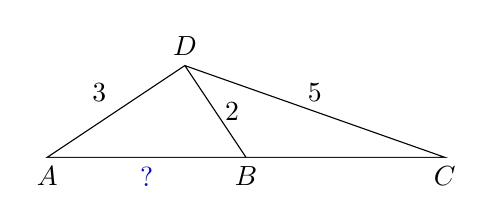
\begin{tikzpicture}[scale=.7]
  \coordinate[label=below:$A$] (A) at ({-sqrt(13)},0);
  \coordinate[label=below:$B$] (B) at (0,0);
  \coordinate[label=below:$C$] (C) at ({sqrt(13)},0);
  \coordinate[label=above:$D$] (D) at ({-4/sqrt(13)},{6/sqrt(13)});
  \draw (C) -- node[above] {$5$} (D)
    -- node[above left] {$3$} (A) -- cycle
    (B) -- node[right] {$2$} (D);
  \draw[blue] (A) -- node[below] {$?$} (B) -- (C);
\end{tikzpicture}
